\chapter{Implementation of Belief Propagation}
The iterative optimization algorithm is belief propagation algorithm.The steps to implement belief propagation is shown in block diagram shown below
\begin{figure}[h]
\begin{center}
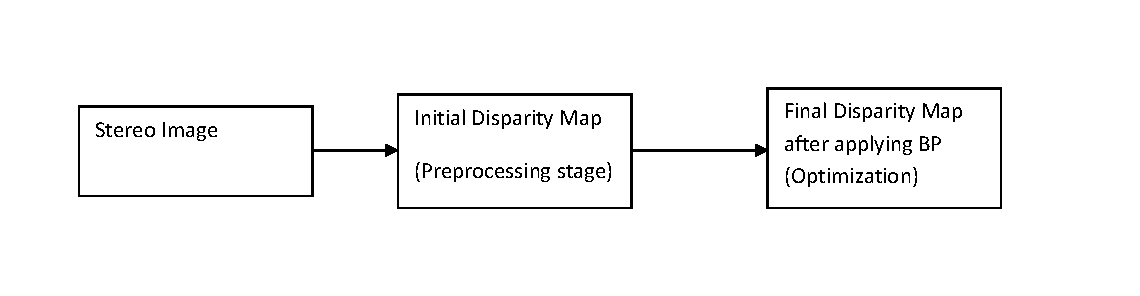
\includegraphics[width=5.5in]{bk.eps}
\caption{Block Diagram for stereo matching technique using Belief Propagation}\label{lined}
\end{center}
\end{figure}
\section{Stereo image(Image rectification)}
The image rectification is to make the epipolar  lines of two camera images aligned horizontally . This can be done by using linear transformations that rotate, translate and skew the camera images.

The principle of image rectification is shown in above figure. The original camera image planes are drawn with solid borders and the rectified image planes are drawn with dashed borders. \newline Epipolar lines are also drawn from the projected points p and p'to epipoles e and e'
After image rectification has been carried out, the epipolar lines of two projected points are parallel and horizontally aligned along the new image planes. The stereo matching problem is therefore reduced to a one dimensional search along horizontal lines instead of a two dimensional search.
\newline Input image referred as a left image corresponding to camera 1, specified in 2-D grayscale. Input image referred as  a right image  corresponding to camera 2 which is also specified in 2-D gray scale. The Input images left and right must be real, finite, and non sparse. They must be the same class.
\begin{figure}[h]
\begin{center}
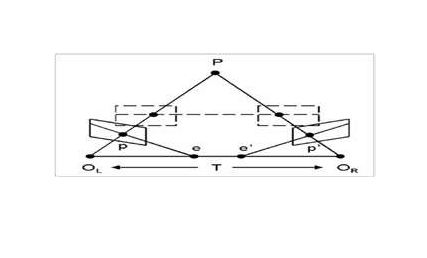
\includegraphics[width=4.5in]{epipolar1.eps}
\caption{Image Rectification}\label{lined}
\end{center}
\end{figure}
\section{Initial Depth Map}
The initial depth map   as a preprocessing  stage  is generated by two methods
\begin{enumerate}
  \item Matlab in build function(DisparityMap)
  \item Minimum Index method
\end{enumerate}
\begin{itemize}
  \item The   DisparityMap  is a  inbuild function in computer vision toolbox of MATLAB. The function DisparityMap finds  disparity  between left and right images.\newline The disparity estimation algorithm used  for DisparityMap function are Semi global and blockmatching he  algorithm. The both disparity estimation algorithm uses the sum of absolute difference(SAD) of each block of pixels  for stereo image. Additionally  in semiglobal disparity estimation it compares similar  disparity on neighboring blocks.\newline The disparity estimation algorithms  also Compute a measure of contrast of the image by using the Sobel filter and Compute the disparity for each pixel in left image.
  \item In minimum index method sum of absolute difference function is used. The disparity or label is fixed to real number either 8 or 16.\newline The intensity values of right image is shifted by a label in column wise, than finding the absolute difference between left and right stereo image. \newline The number of matrix depends on the size of the label or disparity. The next step is finding the minimum shift values as a disparity where minimum occurs
\end{itemize}
\subsection{ Pseudo code for minimum index method}
Left Image =LI of dimension of (M, N)
\newline Right Image =RI of dimension of (M, N)
\newline \%label or disparity is 16
\newline \% Right image matrix is shifted column wise 1 to 16
\newline fori=1:M
\newline for j=16:N     % to avoid overflow
\newline E1(i,j)=abs\{LI(i,j)-RI(i-1,j)\}....... E16(i,j)=abs\{LI(i,j)-RI(i-16,j)\}
\newline \%The shift value as disparity where the minimum occurs.
\newline \%This means if the element of E5 (i,j) gets the minimum value among all (E1 to E16) (Then the disparity value is 5!)shift through column index.
\newline D(i,j)= min{(E1(i,j),E2(i,j),E3(i,j)........E16(i,j))} \newline end \newline end
\section{Belief Propagation Algorithm}
The initial depth map generated either by matlab in build function 'Disparity Map' or by minimum index method is improved by optimization algorithm i.e. Belief Propagation algorithm.
\newline The initial values from initial depth map is normalized between the values $1/16 $to $16/16$.The messages in belief propagation are updated in one movement.The updated messages in one movement means for the right movement. Similarly the up, left, down movements can be executed to complete one iteration.
\subsection{The pseudo code for BP}

for i=1: M   \% in order to avoid the edge effect or index overflow  from 16 to M-16
\newline	for j=1:N \% in order to avoid the edge effect or index overflow from 16 to N-16
\newline	DC(i,j)= abs((LI(i,j)-RI(i -D(i,j),j)/ 256;\% this will be intensity value difference so we normalize by dividing by 256
\newline for k=1:16
\newline	M(k,1)= exp-(DC(i,j)+(abs(D(i-1,j)-(k/16))+ abs(D(i,j+1)-(k/16))+abs(D(i,j-1)-(k/16)));
\% here we have taken the values for right movement part of the loopy propagation
\newline\% for up movement exp-(DC(i,j)+(abs(D(i-1,j)-(k/16))+ abs(D(i+1,j)-(k/16))+ abs(D(i,j-1)-(k/16)))
\newline \% for left movement exp-(DC(i,j)+(abs(D(i+1,j)-(k/16))+ abs(D(i,j+1)-(k/16))+ abs(D(i,j-1)-(k/16)))
\newline \% for down movement exp-(DC(i,j)+(abs(D(i-1,j)-(k/16))+ abs(D(i+1,j)-(k/16))+ abs(D(i,j+1)-(k/16)))
\newline	End \% this completes the generation of message in the sum of product approach
\newline\% Now we need to put the label with the index with maximum value of M.
\newline x=0;
\newline y=0
\newline	fork=1: 16
\newline		if M(k,1)>x
\newline x=M (k,1);
\newline y=k;
\newline end
\newline	end\% at this point 'y' equals index of the max value of the message vector.
\newline	D(i,j)= y/16; \% This action is assigning 'the belief' or the max value of the cost.
	\newline end
\newline end
\section{Results and Conclusion}
The  stereo images for testing are from  data sets 2014 of Middlebury computer vision web site (vision.middlebury.edu)
Aloe vera plant and Lampshade are considered as test stereo images.
\begin{itemize}
  \item Stereo image Aloe Vera(427x370)Size of left image :323KB,Size of right  image :324KB
  \item Stereo image Lamp shade(433x370)Size of left image :172KB,Size of right  image :172KB
\end{itemize}

Initial depth map for test images using matlab in build function 'DisparityMap'and than on applying  Belief Propagation algorithm are  shown

\begin{figure}[h]
\centering
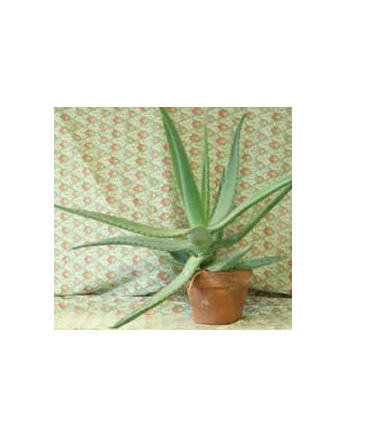
\includegraphics[width=3in]{leftal.eps}
\caption{Aloe vera left stereo image} \label{lined}
\end{figure}

\begin{figure}
\begin{center}
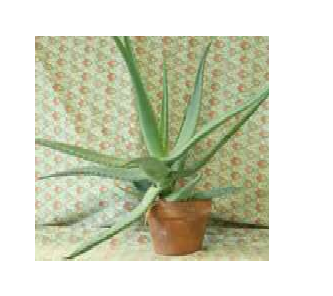
\includegraphics[width=3in]{rightal.eps}
\caption{Aloe vera Right stereo image} \label{lined}
\end{center}
\end{figure}


\begin{figure}[h]
\begin{center}

\includegraphics[width=3in]{idmalma.eps}
\caption{Initial Depth Map using MATLAB Function} \label{lined}
\end{center}
\end{figure}
\begin{figure}[h]
\begin{center}
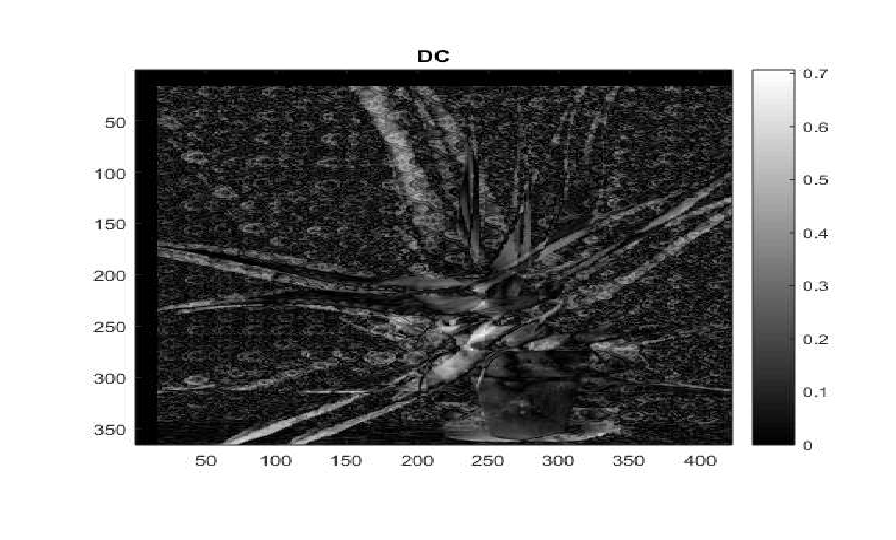
\includegraphics[width=3in]{dmmaal.eps}
\caption{Depth Map after BP} \label{lined}
\end{center}
\end{figure}






\begin{figure}[h]
\begin{center}
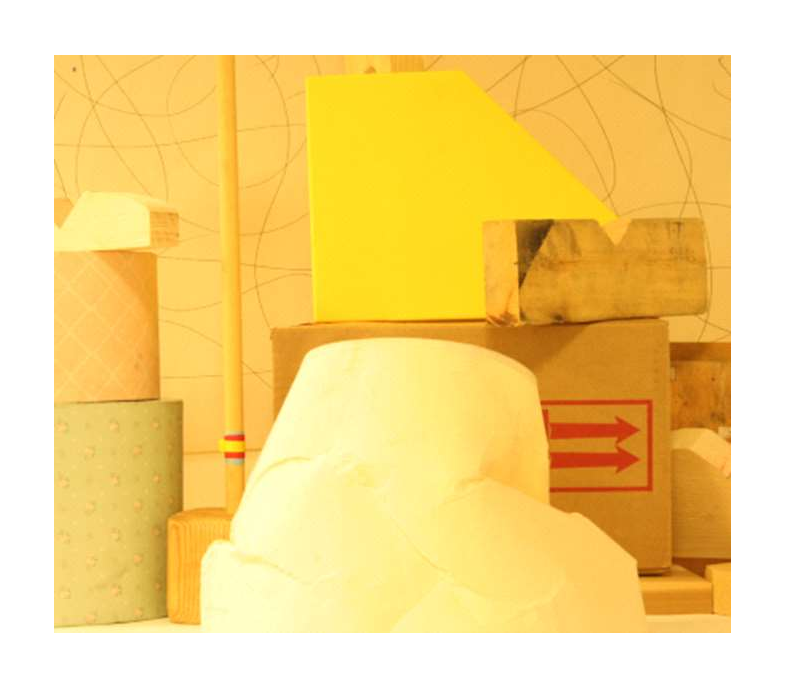
\includegraphics[width=3in]{leftlam.eps}
\caption{Lamp shade left stereo image} \label{lined}
\end{center}
\end{figure}
\begin{figure}[h]
\begin{center}
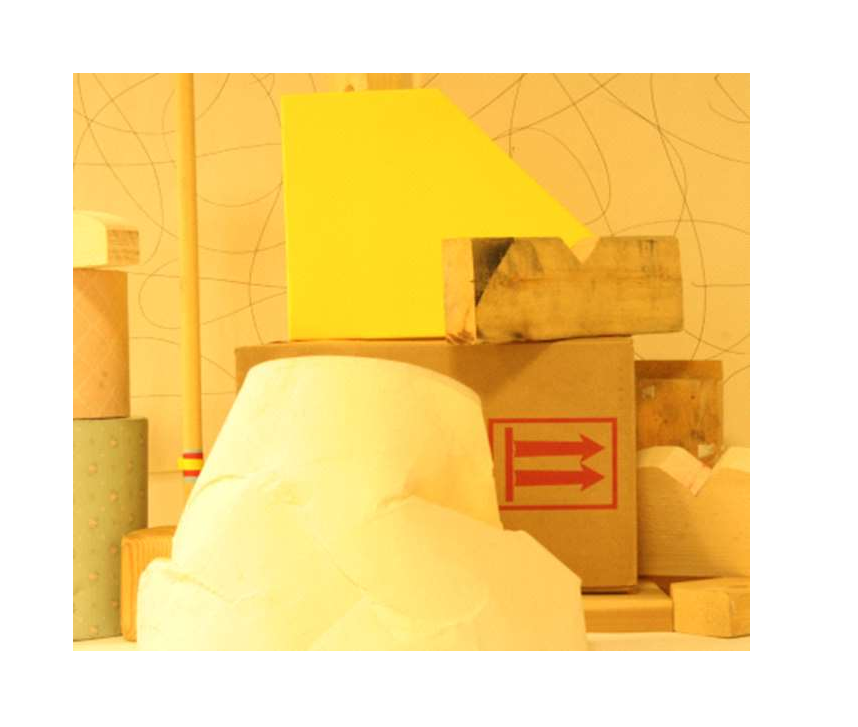
\includegraphics[width=3in]{rightlam.eps}
\caption{Lamp shade Right stereo image} \label{lined}
\end{center}
\end{figure}
\begin{figure}[h]
\begin{center}
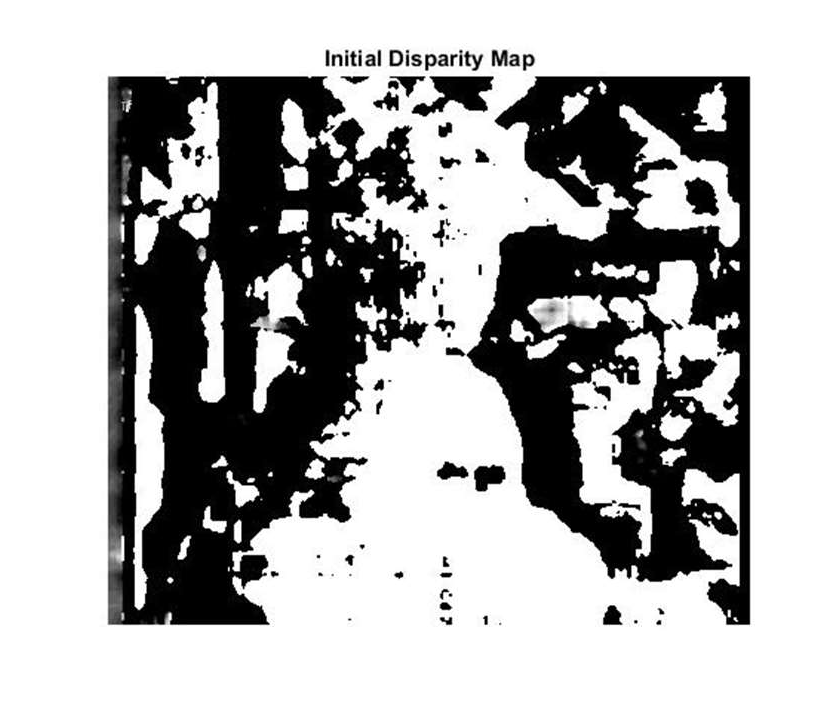
\includegraphics[width=3in]{idmlamma.eps}
\caption{Initial Depth MAP using MATLAB Function for Lamp shade } \label{lined}
\end{center}
\end{figure}
\begin{figure}[h]
\begin{center}
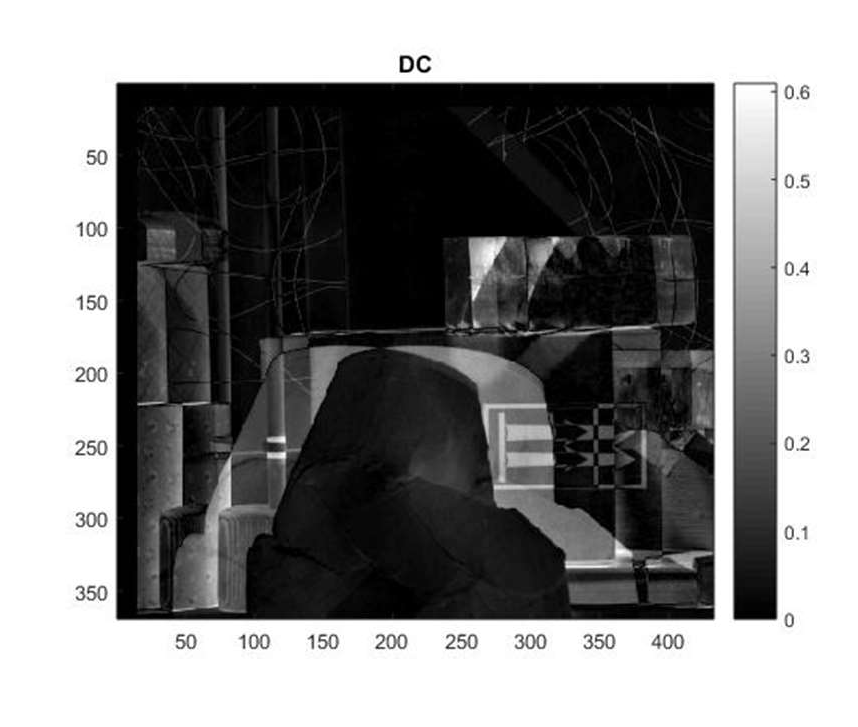
\includegraphics[width=3in]{dmlamma.eps}
\caption{Depth Map after BP for Lamp shade} \label{lined}
\end{center}
\end{figure}
Initial depth map for test images using minimum index method and than on applying  Belief Propagation algorithm are  shown

\begin{figure}[h]
\begin{center}
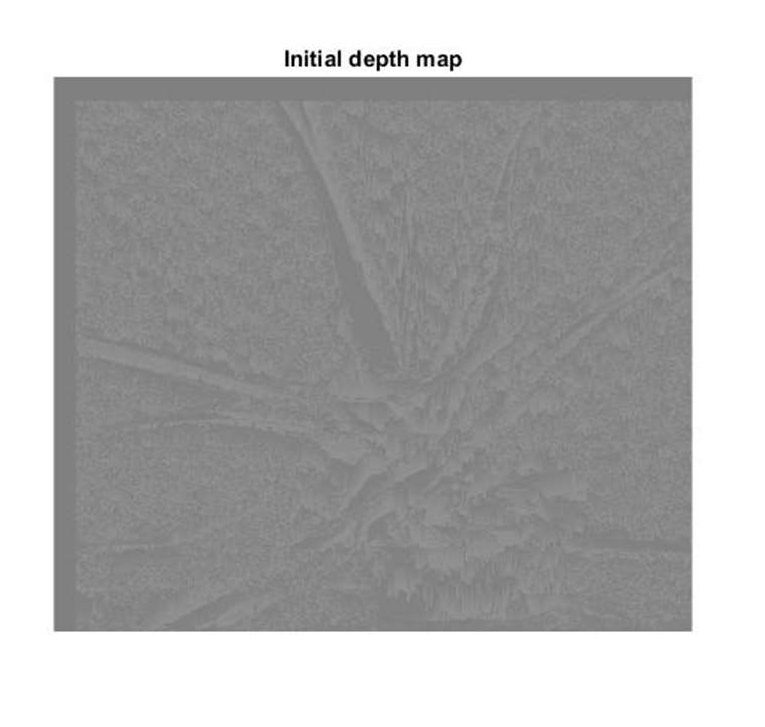
\includegraphics[width=3in]{idmMIal.eps}
\caption{Initial Depth Map using Minimum index method for Aloe vera Plant}\label{lined}
\end{center}
\end{figure}



\begin{figure}[h]
\begin{center}
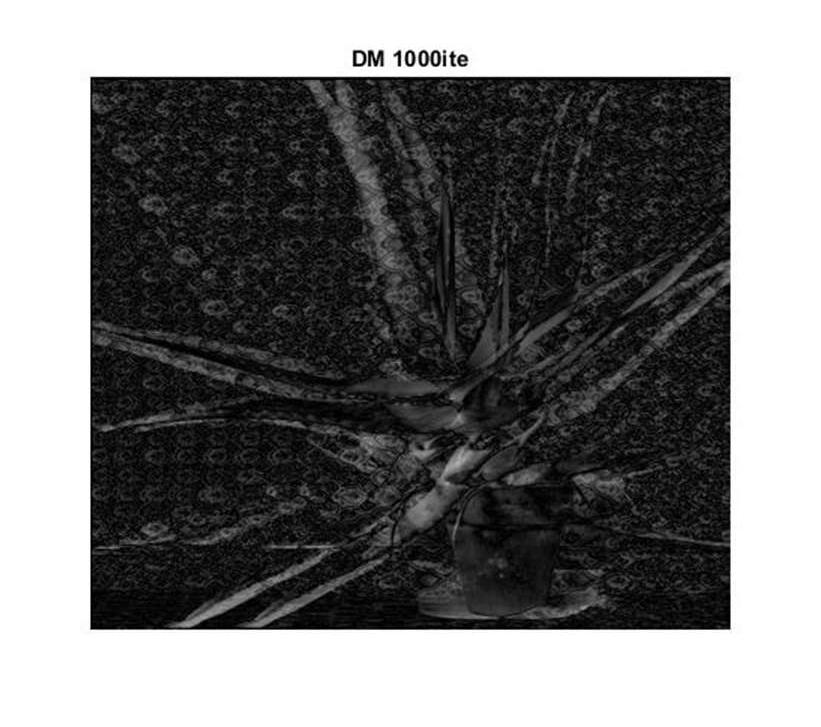
\includegraphics[width=3in]{dmMIal.eps}
\caption{Depth Map after BP for Aloe vera Plant} \label{lined}
\end{center}
\end{figure}
\begin{figure}[h]
\begin{center}
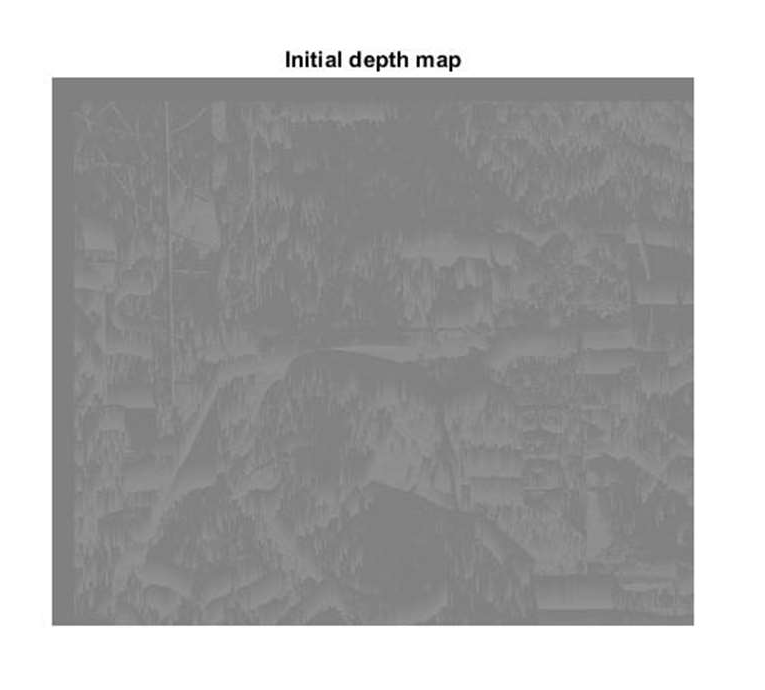
\includegraphics[width=3in]{idmMIlam.eps}
\caption{Initial Depth Map using Minimum index method for Lamp shade} \label{lined}
\end{center}
\end{figure}
\begin{figure}[h]
\begin{center}
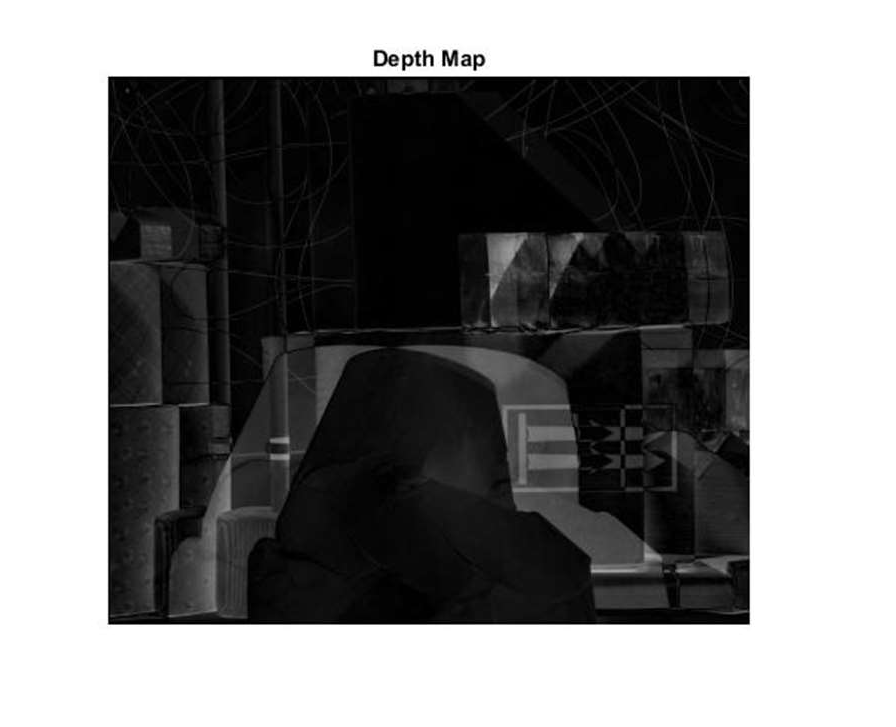
\includegraphics[width=3in]{dmMIlam.eps}
\caption{Depth Map after BP for Lamp shade} \label{lined}
\end{center}
\end{figure} 

